\chapter{Lecture 9 - Pinch-Point Temperature Difference}
\label{ch:ch9}
\section{Objectives}
The objectives of this lecture are:
\begin{itemize}
\item Describe pinch-point temperature difference ($\Delta T_{p}$) and show how to calculate it.
\item Show relationship between $\Delta T_{p}$ and exergy destruction rate in the Steam Generator (SG).
\item Compute $\Delta T_{p}$ for a few modern commercial PWRs.
\item Provide thumb rules/guidance for concept design use.
\end{itemize}

\index{Pinch-Point Temperature Difference}

\section{Description of $\Delta T_{p}$}
\newthought{The pinch-point temperature difference} is the minimum difference between the primary coolant and the secondary coolant in a PWR.  This is shown schematically in the temperature-entropy diagram in Figure \ref{fig:ppdp_TS}. An alternative representation of the process is shown in Figure \ref{fig:ppdp_hx}.
\begin{marginfigure}
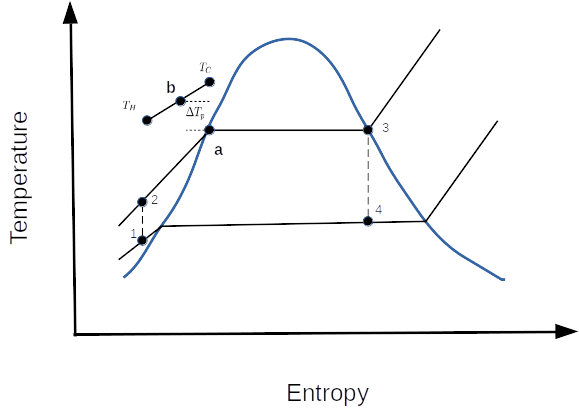
\includegraphics{pinch_point_TS.png}
\caption{Schematic illustration of $\Delta T_{p}$.}
\label{fig:ppdp_TS}
\end{marginfigure}


\begin{marginfigure}
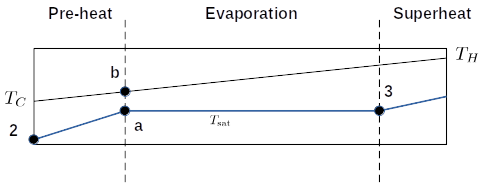
\includegraphics{pinch_point_hx.png}
\caption{Illustration of $\Delta T_{p}$.}
\label{fig:ppdp_hx}
\end{marginfigure}

\newthought{Let us take a moment} to discuss these representations:

\begin{itemize}
\item These representations are not intended to be taken literally.  The SG for most PWRs is, of course, not a once-through counter-flow heat exchanger as Figure \ref{fig:ppdp_hx} indicates.\sidenote{Although in fairness when the concept of $\Delta T_{p}$ was formulated, such SGs were in use and it probably seemed less crazy.} 
\item Consequently, one shouldn't expect to be able to point to the spot on a SG where $\Delta T_{p}$ is realized.
\item Nonetheless, $\Delta T_{p}$ can still be used as a useful engineering parameter because it relates to the relative temperature of the primary coolant and the steam generator. 
\end{itemize}

\newthought{In Heat Transfer class} you will learn one method for analyzing heat exchangers, like the SG, using the log-mean temperature difference. Equation \ref{eq:hx_eq} says that:
\begin{itemize}
\item The rate of heat transfer $(\dot{Q}_{\text{SG}})$ is equal to the product of the overall-heat transfer coefficient $(U)$\marginnote[-1.0cm]{\textbf{Note: }The overall heat transfer coefficient combines the effects conductive heat transfer through heat exchanger surfaces as well as convective heat transfer to/from the heated/cooled fluids.}, the heat transfer surface area $(A)$ and the log-mean temperature difference $(\Delta T_{\text{LM}})$\marginnote[0.25cm]{\textbf{Note: }Log-mean temperature difference is computed based on the difference in temperatures at the heat exchanger inlets and outlets. Specifically, $\Delta T_{\text{LM}} = \frac{\Delta T_{\text{side-a}} - \Delta T_{\text{side-b}}}{\ln{\frac{\Delta T_{\text{side-a}}}{\Delta T_{\text{side-b}}}}}$. Referencing Figure \ref{fig:ppdp_hx}, the log mean temperature difference is calculated as: $\Delta T_{\text{LM}} = \frac{(T_{H}-T_3) - (T_{C} - T_2)}{\ln{\frac{T_{H} - T_3}{T_C - T_2}}}$}; and
\item That heat transfer rate is also equal to the rate of heat transfer into the secondary system water and heat transfer from the primary coolant.
\end{itemize}

\begin{equation}
\dot{Q}_{\text{SG}} = UA\Delta T_{\text{LM}} = \dot{m}_s(h_3 - h_2) = \dot{m}_p(h_{H} - h_{C})
\label{eq:hx_eq}
\end{equation}


\newthought{This is the first time} so far in this course where we have attempted to relate the performance of a heat exchanger to any real-world parameters of the heat exchanger.  In past lectures, heat exchangers like feedwater heaters, SGs, and condensers were represented only as rectangles on a schematic with in-flows and out-flows and some expectation as to what the temperatures of the respective fluids would be.  No consideration was given as to what a heat exchanger would look like; how big it would be, what materials it would be made of, and if the expected performance was in any way realistic.

\newthought{To the extent} that this shortcoming is addressed at all, we do it with the ``Second Law'' exergy analysis.  If the exergy destruction rate is calculated correctly and if the result is negative that is a clear sign that you've laid out impossible expectations for heat exchanger performance.  With this lecture we will establish an additional safe-guard against wishful thinking.  We will calculate $\Delta T_{p}$ and compare it to ``typical'' values achieved for existing designs.  If it is comparable to what currently exists: we can have faith that the specified performance is not crazy.  If the $\Delta T_{p}$ is significantly lower than typical: it is a sign that we will have to do additional analysis to prove that our hopes can realistically be achieved.

\section{Calculating $\Delta T_{p}$}
For the evaluation of $\Delta T_{p}$ we will assume that the following parameters are known: steam or primary coolant mass flow rate; hot- and cold-leg temperature of the primary; temperature of feedwater entering the SG; and the SG pressure or temperature.\sidenote{For purposes of this discussion, we will assume that the steam leaving the SG is saturated vapor.}  The basic energy balance for the SG, using the cycle depicted in Figure \ref{fig:ppdp_TS} is given as:
$$ \dot{m}_p (h_H - h_C) = \dot{m}_s (h_3 - h_2) $$
If we account for the enthalpy of the saturated liquid in the SG $(h_a)$ and the corresponding enthalpy of the primary coolant at the pinch-point $(h_b)$ we can break the energy balance down further:
\begin{align*}
\dot{m}_p(h_b - h_C) &= \dot{m}_s (h_a - h_2) \\
\dot{m}_p(h_H - h_b) &= \dot{m}_s (h_3 - h_a) \\
\end{align*}
Using the first of those equations, we derive an expression for $h_b$:
$$ h_b = \frac{\dot{m}_s}{\dot{m}_p}(h_a - h_2) + h_C$$
If we know $h_b$ and the primary system pressure $(P_{\text{pri}})$ we can find $T_b$.  Using the steam generator pressure and the fact that $h_a$ corresponds to the enthalpy of the saturated liquid, we can find $T_a$ as the saturation temperature for the given SG pressure. Thus:
$$\Delta T_{p} = T_b - T_a$$
\newthought{Pinch-point temperature difference} is directly related to exergy destruction rate in the SG.  Higher $\Delta T_p$ corresponds to higher exergy destruction, more irreversibility, and lower efficiency; lower $\Delta T_p$ corresponds to lower exergy destruction, less irreversibility, and higher plant efficiency.  On the other hand, SGs with lower $\Delta T_p$, all other things being equal, must be larger or made with materials having improved thermal conductivity or have enhanced convective heat transfer performance (or both!).

\newthought{The following guidance} is offered to you for consideration when developing a concept design for a PWR:
\begin{itemize}
\item A reasonable range of $\Delta T_p$ based on historical experience is 20 - 30 degrees Fahrenheit.\cite{rust1979nuclear}
\item Related to the $\Delta T_p$ calculation: the temperature of feedwater for the SG should be approximately 100 degrees F less than saturation temperature in the SG.\cite{el1982nuclear}
\item An analysis of more contemporary PWR designs yield values of $\Delta T_p$ in the range of 18-22 degrees Fahrenheit.
\item In short: around 20 degrees F is a good starting point.
\item If you must make your SG more compact---e.g. developing a PWR-based micro reactor---it is likely that you will need to accept higher values for $\Delta T_p$.
\item If you can afford a very large SG then you can entertain a $\Delta T_p$ lower than 20 degrees F.
\item A reasonable choice of $\Delta T_p$ should give you confidence that a detailed heat exchanger design analysis will show that the heat transfer performance can be achieved with a SG of reasonable size.
\end{itemize}



